% ============================================================
%  Prediction-Based Lossy Compression via DEIM and Gaussian Processes
%  Pitch for SZ researchers — Tuesday meeting  [REVISED]
%  Compile: pdflatex slides_sz_meeting.tex  (run twice)
%  Requires: beamer-theme-metropolis  (tlmgr install beamer-theme-metropolis)
%  Figures must be in the same directory as this .tex file.
% ============================================================
\documentclass[aspectratio=169, 11pt]{beamer}

\usetheme{metropolis}

% ── packages ────────────────────────────────────────────────
\usepackage{booktabs}
\usepackage{colortbl}
\usepackage{amsmath, amssymb, bm}
\usepackage{graphicx}
\usepackage{xcolor}
\usepackage{tikz}
\usepackage[protrusion=true, expansion=false]{microtype}
\usepackage[T1]{fontenc}
\usetikzlibrary{arrows.meta, positioning, fit, backgrounds}

\graphicspath{{./}}

% ── colour palette ──────────────────────────────────────────
\definecolor{cnavy}{HTML}{0D2137}
\definecolor{cteal}{HTML}{1A6B8A}
\definecolor{cice}{HTML}{D6EBF5}
\definecolor{camber}{HTML}{F0A500}
\definecolor{cgreen}{HTML}{1D8A5E}
\definecolor{cred}{HTML}{C0392B}
\definecolor{cmuted}{HTML}{5A7385}
\definecolor{corange}{HTML}{E07B39}

% ── metropolis overrides ────────────────────────────────────
\setbeamercolor{normal text}{fg=cnavy, bg=white}
\setbeamercolor{frametitle}{bg=cnavy, fg=white}
\setbeamercolor{title separator}{fg=cteal}
\setbeamercolor{progress bar}{fg=cteal, bg=cice}
\setbeamercolor{alerted text}{fg=camber}
\setbeamercolor{block title}{bg=cice, fg=cnavy}
\setbeamercolor{block body}{bg=cice!40, fg=cnavy}
\setbeamercolor{itemize item}{fg=cteal}
\setbeamercolor{itemize subitem}{fg=cmuted}
\setbeamercolor{enumerate item}{fg=cteal}
\setbeamerfont{frametitle}{size=\large, series=\bfseries}
\setbeamerfont{block title}{series=\bfseries, size=\small}
\setbeamerfont{block body}{size=\small}

% ── placeholder for missing figures ─────────────────────────
\newcommand{\figplaceholder}[2][0.85\linewidth]{%
  \fbox{\parbox{#1}{\centering\vspace{1.8cm}%
    \textcolor{cmuted}{\small\textit{[#2]}}\vspace{1.8cm}}}}

% ── title info ───────────────────────────────────────────────
\title{Prediction-Based Lossy Compression\\via DEIM and Gaussian Processes}
\subtitle{A sensor-driven predictor framework for structured scientific data}
\author{Jessie Chen}
\institute{Argonne National Laboratory}
\date{August 2026}

% ============================================================
\begin{document}
% ============================================================

% ── SLIDE 1: Title ──────────────────────────────────────────
\maketitle

% ── SLIDE 2: Motivation ─────────────────────────────────────
\begin{frame}{Why Better Predictors?}
\begin{columns}[T]

\begin{column}{0.52\textwidth}
  \textcolor{cteal}{\textbf{Prediction is the main component in prediction-based compression}}\vspace{0.3em}
  \begin{itemize}\setlength\itemsep{0.3em}\small
    \item SZ's Lorenzo predictor uses a \textbf{local finite-difference stencil} --- it looks at each data point's immediate neighbors, one value at a time
    \item Many scientific datasets (ocean, atmosphere, climate) have \textbf{strong global spatial correlations} --- the same large-scale patterns repeat across time
    \item \textbf{Question:} can a predictor that sees the whole domain at once --- rather than one point at a time --- produce smaller residuals?
  \end{itemize}

  \vspace{0.5em}
  \textcolor{cteal}{\textbf{This work}}\vspace{0.2em}\\
  \small We test two global regression methods --- DEIM and Gaussian Processes --- as drop-in preprocessors before SZ2, and measure whether the smaller residuals translate to better rate-distortion.
\end{column}

\begin{column}{0.44\textwidth}
  \vspace{0.5em}
  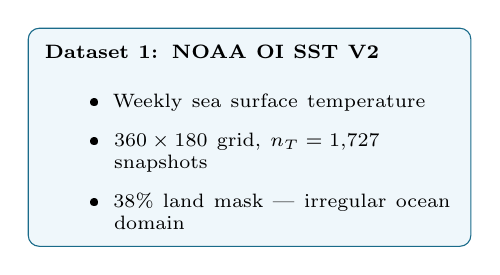
\begin{tikzpicture}
    \node[draw=cteal, rounded corners, fill=cice!40, inner sep=6pt, text width=5.2cm] (box) {
      \scriptsize
      \textbf{Dataset 1: NOAA OI SST V2}\\[3pt]
      \begin{itemize}\setlength\itemsep{2pt}
        \item Weekly sea surface temperature
        \item $360 \times 180$ grid, $n_T = 1{,}727$ snapshots
        \item 38\% land mask \textemdash{} irregular ocean domain
%        \item Strong global spatial correlations; rapid singular value decay
      \end{itemize}
    };
  \end{tikzpicture}

  \vspace{0.5em}
  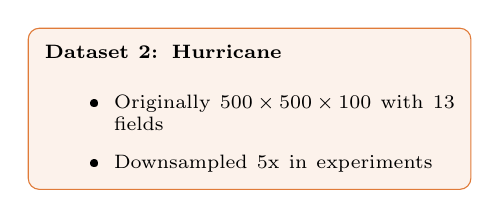
\begin{tikzpicture}
    \node[draw=corange, rounded corners, fill=corange!10, inner sep=6pt, text width=5.2cm] {
      \scriptsize
      \textbf{Dataset 2: Hurricane}\\[3pt]
      \begin{itemize}\setlength\itemsep{2pt}
        \item Originally  $500 \times 500 \times 100$ with 13 fields
%        \item Sharper gradients; more localized structures
        \item Downsampled 5x in experiments
      \end{itemize}
    };
  \end{tikzpicture}
\end{column}

\end{columns}
\end{frame}

% ── SLIDE 3: DEIM + GP high-level intro ─────────────────────
\begin{frame}{Global Regression Preprocessors: DEIM and GP}
\begin{columns}[T]

\begin{column}{0.50\textwidth}
  \textcolor{cteal}{\textbf{The core idea}}\vspace{0.25em}
  \begin{itemize}\setlength\itemsep{0.35em}\small
    \item \textbf{Train once} on representative snapshots --- learn the global spatial correlation structure of the field
    \item At compression time, \textbf{read $k$ sensor values} and regress the full field from them
    \item Unlike SZ: prediction is a \textbf{single global operation} over the whole domain, not datapoint-by-datapoint
  \end{itemize}
\end{column}

\begin{column}{0.46\textwidth}
  \begingroup
  \setbeamercolor{block title}{bg=camber!20, fg=cnavy}
  \setbeamercolor{block body}{bg=camber!10, fg=cnavy}
  \begin{block}{DEIM}
    \scriptsize
    Learns a low-rank basis (SVD) from training snapshots.
    Selects sensor locations algebraically (Q-DEIM).
    Reconstructs via linear interpolation in the basis.\\[2pt]
    \textbf{Model size:} $\sim$30\,MB (basis matrix, stored once).
  \end{block}
  \endgroup

  \vspace{0.4em}
  \begingroup
  \setbeamercolor{block title}{bg=cgreen!20, fg=cnavy}
  \setbeamercolor{block body}{bg=cgreen!10, fg=cnavy}
  \begin{block}{Gaussian Process (Kriging)}
    \scriptsize
    Fits a spatial covariance model (Mat\'{e}rn kernel) via MLE.
    Selects sensor locations via RPCholesky.
    Reconstructs via GP posterior mean --- a global kernel regression.\\[2pt]
    \textbf{Model size:} $\sim$80\,KB (hyperparams only; no basis stored).
  \end{block}
  \endgroup
\end{column}

\end{columns}
\end{frame}

% ── SLIDE 4: DEIM visual ────────────────────────────────────
\begin{frame}{What DEIM Produces}
%\begin{columns}[T]
%
%\begin{column}{0.60\textwidth}
%  \begin{center}
%    \includegraphics[width=0.8\linewidth]{deim_showcase.png}
%  \end{center}
%\end{column}
%
%\begin{column}{0.36\textwidth}
%  \vspace{1.0em}
%  \begin{itemize}\setlength\itemsep{0.45em}\small
%    \item From only $k=800$ sensor readings out of $42{,}376$ ocean pixels, DEIM recovers the global temperature pattern
%    \item The basis $\boldsymbol{\Phi}_k$ is trained once; each new snapshot requires only a small linear solve
%    \item Singular values of the SST anomaly matrix decay rapidly --- a small basis suffices
%  \end{itemize}
%\end{column}
%
%\end{columns}

  \begin{center}
    \includegraphics[width=0.9\linewidth]{recon_panel_DEIM_Hurricane.png}
  \end{center}
\end{frame}

% ── SLIDE 5: GP visual ──────────────────────────────────────
\begin{frame}{What Gaussian Process Kriging Produces}
\begin{center}
  \includegraphics[width=0.9\linewidth]{recon_panel_SST.png}\\[0.3em]
  \scriptsize
  \textbf{Left:} GP posterior mean prediction \quad
  \textbf{center:} pointwise error \quad
  \textbf{Right:} sensor locations ($\times$) chosen by RPCholesky
\end{center}
\end{frame}

% ── SLIDE 5b: Visual Quality (moved here from after RD results) ─────────────
\begin{frame}{Visual Quality --- SST}

  \begin{center}
    \includegraphics[width=0.75\linewidth]{poster_field_panel_SST.png}\\
    \scriptsize True SST \;|\; DEIM recon \;|\; GP recon \;|\; Residual histograms
  \end{center}

\end{frame}

% ── SLIDE 5c: Prediction residual diagnostic ────────────────
\begin{frame}{Isolating the Prediction Step: Lorenzo vs DEIM vs GP}
\begin{columns}[T]

\begin{column}{0.5\textwidth}
  \begin{center}
  \IfFileExists{lorenzo_vs_global_residuals.png}{%
    \includegraphics[width=\linewidth]{lorenzo_vs_global_residuals.png}%
  }{%
    \figplaceholder{lorenzo\_vs\_global\_residuals.png}%
  }
  \end{center}
\end{column}

\begin{column}{0.29\textwidth}
  \vspace{0.8em}
  \textcolor{cteal}{\textbf{Key observations}}\vspace{0.3em}
  \begin{itemize}\setlength\itemsep{0.4em}\scriptsize
    \item Pure prediction comparison --- \textbf{no compression}
    \item Lorenzo uses immediate neighbors
    \item DEIM and GP use $k$ sparse sensors 
    \item Quality varies with number of sensors
  \end{itemize}
\end{column}

\end{columns}
\end{frame}

% ── SLIDE 6: Residual motivation ────────────────────────────
\begin{frame}{Global Approximation is Good --- But Not Perfect Locally}
\begin{columns}[T]

\begin{column}{0.52\textwidth}
  \textcolor{cteal}{\textbf{What the error map shows}}\vspace{0.3em}
  \begin{itemize}\setlength\itemsep{0.35em}\small
    \item The global prediction captures the dominant spatial pattern well --- overall PSNR is high
    \item But local residuals are \textbf{non-zero and spatially structured}: the model under- or over-estimates in patches
    \item These structured residuals are exactly what SZ2 and ZFP are designed to compress efficiently
  \end{itemize}

  \vspace{0.5em}
  \textcolor{cteal}{\textbf{Natural division of labour}}\vspace{0.3em}
  \begin{itemize}\setlength\itemsep{0.35em}\small
    \item \textbf{DEIM / GP:} handle the global structure
    \item \textbf{SZ2:} handle the remaining local residual
  \end{itemize}
\end{column}

\begin{column}{0.44\textwidth}
  \vspace{0.5em}
  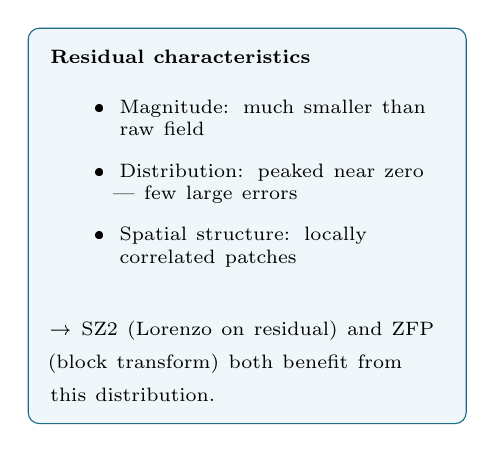
\begin{tikzpicture}
    \node[draw=cteal, rounded corners, fill=cice!40, inner sep=8pt, text width=5.0cm] {
      \scriptsize
      \textbf{Residual characteristics}\\[4pt]
      \begin{itemize}\setlength\itemsep{3pt}
        \item Magnitude: much smaller than raw field
        \item Distribution: peaked near zero --- few large errors
        \item Spatial structure: locally correlated patches
      \end{itemize}
      \vspace{4pt}
      \textrightarrow{} SZ2 (Lorenzo on residual) and ZFP (block transform) both benefit from this distribution.
    };
  \end{tikzpicture}
\end{column}

\end{columns}
\end{frame}

% ── SLIDE 7: SZ3 Framework ──────────────────────────────────
\begin{frame}{Where DEIM / GP Fits in the SZ3 Pipeline}
\small
\vspace{0.2em}

\begin{center}
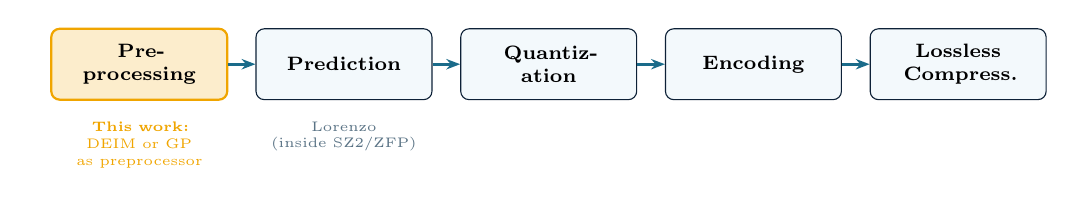
\begin{tikzpicture}[
  box/.style={draw=cnavy, rounded corners=3pt, minimum height=0.9cm,
              text width=2.0cm, align=center, font=\scriptsize\bfseries, fill=cice!30},
  arrow/.style={-{Stealth[length=5pt]}, line width=1.2pt, color=cteal},
  highlight/.style={draw=camber, rounded corners=3pt, minimum height=0.9cm,
                    text width=2.0cm, align=center, font=\scriptsize\bfseries,
                    fill=camber!20, thick}
]
  \node[highlight] (pre)  at (0,0)   {Pre-\\processing};
  \node[box]       (pred) at (2.6,0) {Prediction};
  \node[box]       (quant)at (5.2,0) {Quantiz-\\ation};
  \node[box]       (enc)  at (7.8,0) {Encoding};
  \node[box]       (lc)   at (10.4,0){Lossless\\Compress.};

  \draw[arrow] (pre)   -- (pred);
  \draw[arrow] (pred)  -- (quant);
  \draw[arrow] (quant) -- (enc);
  \draw[arrow] (enc)   -- (lc);

  \node[text width=2.6cm, align=center, font=\tiny, color=camber, below=0.15cm of pre]
    {\textbf{This work:}\\DEIM or GP\\as preprocessor};

  \node[text width=2.4cm, align=center, font=\tiny, color=cmuted, below=0.15cm of pred]
    {Lorenzo\\(inside SZ2/ZFP)};
\end{tikzpicture}
\end{center}

\vspace{0.4em}

\begin{columns}[T]
\begin{column}{0.48\textwidth}
  \begingroup
  \setbeamercolor{block title}{bg=cmuted!20, fg=cnavy}
  \setbeamercolor{block body}{bg=cmuted!10, fg=cnavy}
  \begin{block}{SZ2/ZFP baseline}
    \scriptsize
    No preprocessing step. SZ2 uses a local Lorenzo stencil as its predictor;
    ZFP uses block floating-point transforms.\\[3pt]
    \textbf{Strength:} no training, universal.\\
    \textbf{Weakness:} ignores global spatial modes.
  \end{block}
  \endgroup
\end{column}

\begin{column}{0.48\textwidth}
  \begingroup
  \setbeamercolor{block title}{bg=cgreen!15, fg=cgreen}
  \setbeamercolor{block body}{bg=cgreen!5, fg=cnavy}
  \begin{block}{This work (DEIM / GP preprocessor)}
    \scriptsize
    Add a global preprocessing step \emph{before} SZ2 or ZFP.
    DEIM or GP reconstructs each snapshot from $k$ sensor measurements;
    the residual is then compressed by the full SZ2 pipeline.\\[3pt]
    Lorenzo still runs inside SZ2 --- on a much smaller residual.
  \end{block}
  \endgroup
\end{column}
\end{columns}
\end{frame}

% ── SLIDE 6: Four Methods ───────────────────────────────────
\begin{frame}{Four Methods Under Comparison}
\small
\vspace{0.3em}

\renewcommand{\arraystretch}{1.4}
\scriptsize
\begin{tabular}{p{2.4cm} p{3.2cm} p{2.6cm} p{4.0cm}}
\toprule
\rowcolor{cnavy}
\textcolor{white}{\textbf{Method}} &
\textcolor{white}{\textbf{Predictor}} &
\textcolor{white}{\textbf{Residual encoder}} &
\textcolor{white}{\textbf{Stored bytes}} \\
\midrule
SZ2 (baseline)
  & Lorenzo (local stencil)
  & Huffman + Zstd
  & quantized residuals \\
\rowcolor{cice!40}
ZFP (baseline)
  & Block floating-point
  & Fixed-rate bitstream
  & bitstream \\
\midrule
\rowcolor{camber!20}
DEIM-2D+SZ2
  & DEIM ($k$ modes, Q-DEIM sensors)
  & SZ2 on ocean residual
  & $\Phi_k$ + sensors + vals + SZ2(res) \\
\rowcolor{camber!10}
Kriging-2D+SZ2
  & GP (Mat\'{e}rn, RPCholesky sensors)
  & SZ2 on ocean residual
  & hyperparams + sensors + vals + SZ2(res) \\
\bottomrule
\end{tabular}

\vspace{0.5em}
\small
\textcolor{camber}{\textbf{Amber rows}} use the DEIM or GP global prediction as a preprocessor, then compress the residual with SZ2. ZFP was also tested as an alternative residual encoder but showed no advantage over SZ2 for these residuals.
\end{frame}

% ── SLIDE 7: Setup — SST ────────────────────────────────────
\begin{frame}{Experimental Setup --- SST}
\begin{columns}[T]

\begin{column}{0.48\textwidth}
  \textcolor{cteal}{\textbf{NOAA OI SST V2}}\vspace{0.2em}
  \begin{itemize}\setlength\itemsep{0.3em}\small
    \item $1{,}727$ weekly means, $180\times360$ grid ($\approx$448\,MB)
    \item Ocean mask: $n_\text{ocean} = 42{,}376$ pixels (62\% of grid)
    \item DEIM/GP operate on ocean pixels only
  \end{itemize}

  \vspace{0.6em}
  \textcolor{cteal}{\textbf{Quality metric}}\vspace{0.2em}
  \begin{itemize}\setlength\itemsep{0.3em}\small
    \item PSNR: $20\log_{10}\!\bigl(\tfrac{\max-\min}{\mathrm{RMSE}}\bigr)$ over all pixels and time steps
  \end{itemize}
\end{column}

\begin{column}{0.48\textwidth}
  \textcolor{cteal}{\textbf{Sensor / mode counts}}\vspace{0.2em}
  \begin{itemize}\setlength\itemsep{0.3em}\small
    \item DEIM: $k \in \{400,\,800,\,1200,\,1600\}$
    \item GP: $k \in \{400,\,800,\,1200,\,1600,\,2000\}$
  \end{itemize}

  \vspace{0.6em}
  \textcolor{cteal}{\textbf{Error bound sweep}}\vspace{0.2em}
  \begin{itemize}\setlength\itemsep{0.3em}\small
    \item $\varepsilon \in [10^{-4},\,1]$, 20 log-spaced values, all 4 methods
    \item Each $(k,\varepsilon)$ pair produces one (CR, PSNR) point
  \end{itemize}
\end{column}

\end{columns}
\end{frame}

% ── SLIDE 8: SST RD Results ─────────────────────────────────
\begin{frame}{Rate-Distortion --- SST (Dataset 1)}
\begin{columns}[T]

\begin{column}{0.60\textwidth}
  \begin{center}
    \includegraphics[width=\linewidth]{rd_psnr_cr_SST.png}
  \end{center}
\end{column}

\begin{column}{0.36\textwidth}
  \vspace{1.0em}
  \textcolor{cteal}{\textbf{Key observations}}\vspace{0.3em}
  \begin{itemize}\setlength\itemsep{0.35em}\small
%    \item At matched CR, DEIM and GP methods achieve \textbf{higher PSNR} than SZ2 and ZFP
    \item GP model overhead $\approx$80\,KB --- negligible relative to dataset
%    \item ZFP was tested as an alternative residual encoder but showed no advantage over SZ2 on these residuals
    \item Shaded region: CR range where one of the hybrid methods exceed the SZ2-1D baseline
  \end{itemize}
\end{column}

\end{columns}
\end{frame}

% ── SLIDE: Setup — Hurricane ────────────────────────────────
\begin{frame}{Experimental Setup --- Hurricane}
\begin{columns}[T]

\begin{column}{0.48\textwidth}
  \textcolor{corange}{\textbf{ISABEL Hurricane (TC)}}\vspace{0.2em}
  \begin{itemize}\setlength\itemsep{0.3em}\small
    \item $100$ vertical levels, $500\times500$ grid ($\approx$100\,MB)
    \item No land mask --- all 250{,}000 pixels active
    \item Dynamic range $\approx 60\,^\circ$C; sharp gradients near storm eye
  \end{itemize}

  \vspace{0.6em}
  \textcolor{corange}{\textbf{Key constraint}}\vspace{0.2em}
  \begin{itemize}\setlength\itemsep{0.3em}\small
    \item SVD rank $\leq n_T = 100$ caps DEIM at $k \leq 80$
    \item 80 modes for a $500\times500$ field is a very thin basis
  \end{itemize}
\end{column}

\begin{column}{0.48\textwidth}
  \textcolor{corange}{\textbf{Sensor / mode counts}}\vspace{0.2em}
  \begin{itemize}\setlength\itemsep{0.3em}\small
    \item DEIM: $k \in \{10,\,20,\,40,\,60,\,80\}$ (hard cap at 80)
    \item GP: $k \in \{50,\,100,\,200,\,400\}$
  \end{itemize}

  \vspace{0.6em}
  \textcolor{corange}{\textbf{Error bound sweep}}\vspace{0.2em}
  \begin{itemize}\setlength\itemsep{0.3em}\small
    \item Same $\varepsilon \in [10^{-4},\,1]$, 20 log-spaced values
  \end{itemize}
\end{column}

\end{columns}
\end{frame}

% ── SLIDE 10: Hurricane RD Results ──────────────────────────
\begin{frame}{Rate-Distortion --- Hurricane (Dataset 2)}

  \begin{center}
    \IfFileExists{poster_rd_psnr_Hurricane.png}{%
      \includegraphics[width=0.65\linewidth]{poster_rd_psnr_Hurricane.png}%
    }{%
      \figplaceholder{poster\_rd\_psnr\_Hurricane.png}%
    }
  \end{center}

\end{frame}

% ── SLIDE 11: Hurricane Field Panel / Multi-GP ──────────────
%\begin{frame}{Visual Quality --- Hurricane (Multi-GP Focus)}
%\begin{columns}[T]
%
%\begin{column}{0.55\textwidth}
%  \begin{center}
%    \IfFileExists{poster_field_panel_Hurricane.png}{%
%      \includegraphics[width=\linewidth]{poster_field_panel_Hurricane.png}%
%    }{%
%      \figplaceholder{poster\_field\_panel\_Hurricane.png}%
%    }
%    \scriptsize True field \;|\; DEIM recon \;|\; GP recon \;|\; Residuals
%  \end{center}
%\end{column}
%
%\begin{column}{0.41\textwidth}
%  \begin{center}
%    \IfFileExists{recon_panel_GP_Hurricane.png}{%
%      \includegraphics[width=\linewidth]{recon_panel_GP_Hurricane.png}%
%    }{%
%      \figplaceholder{recon\_panel\_GP\_Hurricane.png}%
%    }
%    \scriptsize GP prediction, error map, sensor locations
%  \end{center}
%
%  \vspace{0.4em}
%  \small\textcolor{cteal}{\textbf{Multi-GP focus:}} RPCholesky sensor placement adapts to the hurricane's correlation structure. Expect sensors to concentrate near high-variance regions (eye wall, spiral bands).
%\end{column}
%
%\end{columns}
%\end{frame}

% ── SLIDE 12: Storage Budget ────────────────────────────────
\begin{frame}{Where Do the Bytes Go? --- SST at $k=800$}
\begin{columns}[T]

\begin{column}{0.60\textwidth}
  \begin{center}
    \includegraphics[width=\linewidth]{rd_budget_breakdown_SST.png}
  \end{center}
\end{column}

\begin{column}{0.36\textwidth}
  \vspace{0.8em}
  \textcolor{cteal}{\textbf{Budget breakdown}}\vspace{0.3em}
  \begin{itemize}\setlength\itemsep{0.35em}\small
    \item \textbf{DEIM model:} basis $\Phi_k$ (float16) $\approx$30--35\,MB after compression; amortised over $n_T$ snapshots
    \item \textbf{GP model:} hyperparams $\approx$80\,KB total 
    \item \textbf{Sensor values:} $k$ float16 per snapshot; grows with $k$
    \item \textbf{Residuals:} dominant at high-fidelity settings; shrinks as prediction improves or $k$ increases
  \end{itemize}
\end{column}

\end{columns}
\end{frame}

% ── SLIDE 13: Discussion ────────────────────────────────────
\begin{frame}{Discussion}
\begin{columns}[T]

\begin{column}{0.48\textwidth}
  \textcolor{cteal}{\textbf{Strengths}}\vspace{0.2em}
  \begin{itemize}\setlength\itemsep{0.3em}\small
    \item Exploits low-rank global structure in a principled way
    \item Modular: GP and DEIM slots into SZ3 as a \emph{preprocessor module}
    \item DEIM (deterministic) and GP (probabilistic) offer different trade-offs
%    \item Residual encoder interchangeable --- SZ2 or ZFP
%    \item Training is checkpointed; cost amortised over many compressions
  \end{itemize}
\end{column}

\begin{column}{0.48\textwidth}
  \textcolor{cteal}{\textbf{Limitations}}\vspace{0.2em}
  \begin{itemize}\setlength\itemsep{0.3em}\small
%    \item Methods \textbf{do not beat SZ2 on hurricane}: $n_T = 100$ caps DEIM modes; sharp gradients break global smoothness assumption
    \item On SST, gain only appears at \textbf{larger error bounds} --- model overhead dominates at high fidelity
    \item DEIM basis has a large overhead
    \item Training required
  \end{itemize}
\end{column}

\end{columns}
\end{frame}

% ── SLIDE 14: Conclusion ────────────────────────────────────
\begin{frame}{Conclusion \& Next Steps}
\begin{columns}[T]

\begin{column}{0.54\textwidth}
  \textcolor{cteal}{\textbf{Summary}}\vspace{0.2em}
  \begin{itemize}\setlength\itemsep{0.25em}\small
    \item GP / DEIM as a \textbf{preprocessing module} in the SZ3 pipeline
    \item Kriging+SZ2 beat SZ2 on SST at large error bounds
    \item Model overhead negligible ($\sim$80\,KB)
  \end{itemize}

  \vspace{0.4em}
  \textcolor{cteal}{\textbf{Next steps}}\vspace{0.2em}
  \begin{itemize}\setlength\itemsep{0.25em}\small
    \item Integrate as a formal SZ3 predictor module
%    \item Test on datasets with larger $n_T$ and smoother fields
    \item Better quantizers suited to the GP/DEIM residual distribution?
  \end{itemize}
\end{column}

\begin{column}{0.42\textwidth}
  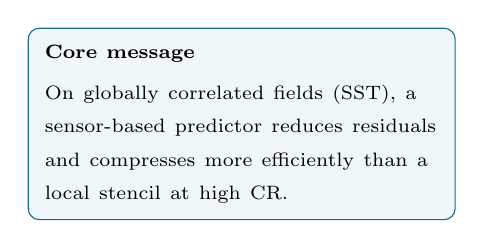
\begin{tikzpicture}
    \node[draw=cteal, rounded corners, fill=cice!40, inner sep=6pt, text width=5.0cm] {
      \scriptsize
      \textbf{Core message}\\[3pt]
      On globally correlated fields (SST), a sensor-based predictor reduces residuals and compresses more efficiently than a local stencil at high CR.
    };
  \end{tikzpicture}

  \vspace{0.4em}
  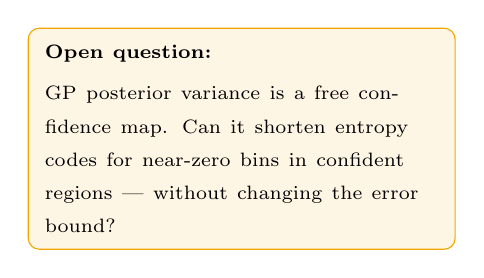
\begin{tikzpicture}
    \node[draw=camber, rounded corners, fill=camber!10, inner sep=6pt, text width=5.0cm] {
      \scriptsize
      \textbf{Open question:}\\[3pt]
      GP posterior variance is a free confidence map. Can it shorten entropy codes for near-zero bins in confident regions --- without changing the error bound?
    };
  \end{tikzpicture}
\end{column}

\end{columns}
\end{frame}

% ============================================================
\end{document}
